\documentclass{article}
\usepackage{graphicx}
\usepackage{amsmath}
\usepackage{hyperref}
\usepackage{biblatex}
\addbibresource{bib.bib}
\usepackage[margin=0.75in]{geometry}
\usepackage{mathptmx}
\usepackage{titlesec}
\usepackage{wasysym}
\usepackage{pifont}
\usepackage[final]{changes}

\usepackage{hyperref}
\hypersetup{
    colorlinks=true,        % Use colored text for links (true) or put a border around them (false)
    linkcolor=black,         % Color for internal links (sections, etc.)
    citecolor=black,        % Color for citations
    urlcolor=black,           % Color for URLs
    pdfborder={0 0 0}       % No border around the links
}

%\usepackage{bbding}
%
%. FORMAT SECTION HEADINGS
%
\titleformat*{\section}{\normalfont\bfseries}
\titleformat*{\subsection}{\normalfont\bfseries}
\titleformat*{\subsubsection}{\normalfont\bfseries}

\titlespacing\section{0pt}{12pt plus 4pt minus 2pt}{0pt plus 2pt minus 2pt}
\titlespacing\subsection{0pt}{12pt plus 4pt minus 2pt}{0pt plus 2pt minus 2pt}
\titlespacing\subsubsection{0pt}{12pt plus 4pt minus 2pt}{0pt plus 2pt minus 2pt}

%
% FORMAT Paragraph / main text
%
\setlength\parindent{0pt}

%
% SET UP HEADER AND FOOTER
%
\usepackage{fancyhdr}
\pagestyle{fancy}
\fancyhf{}
\renewcommand{\headrulewidth}{0pt}
\lhead{} 
\rhead{Dr. James R. Wallace}
\pagenumbering{gobble}
\cfoot{\thepage}

%
% TABLE FORMATTING
%
\usepackage{multirow}
%\usepackage[table,xcdraw]{xcolor}
\usepackage{booktabs}
\usepackage{enumitem}


\title{Salary Discrepancies Between MHI- and Non-MHI-Affiliated \\ Faculty Members in SPHS}
\author{Jim Wallace}
\date{March 2024}

\begin{document}

\maketitle

\section{Data Collection}

To investigate potential salary discrepancies between faculty members affiliated with the Master of Health Informatics (MHI) program and those who are not (non-MHI) at the University of Waterloo, data was collected from the following sources: University of Waterloo public salary disclosures 2011--2024 \cite{uw_salary_2011, uw_salary_2012, uw_salary_2013, uw_salary_2014, uw_salary_2015, uw_salary_2016, uw_salary_2017, uw_salary_2018, uw_salary_2019, uw_salary_2020, uw_salary_2021, uw_salary_2022, uw_salary_2023, uw_salary_2024}, faculty association publications outlining salary structures \cite{fauw_salary_structure}, and School of Public Health Sciences faculty listings \cite{uwaterloo_mhi_faculty}. The data included annual salary figures, MHI affiliation status, and spanned a ten-year period to enable a longitudinal analysis of salary progression.


\section{Analysis}

Faculty members were categorized into two groups based on their MHI affiliation status. Average salary increases over the ten-year period were then computed for each group. Because the dataset represents the full population of faculty in the department, formal statistical inference was not required. Instead, descriptive comparisons and trend visualizations were used to illustrate the observed differences.


\section{Results}

The analysis reveals a notable disparity in salary progression. Non-MHI faculty members experienced an average annual salary increase of approximately \$3,074, whereas MHI-affiliated faculty members saw a lower average of around \$1,541 per year. Over a ten-year span, this resulted in a cumulative difference of approximately \$15,330 in favour of non-MHI faculty. This disparity is consistent with a hypothesis of systemic bias in performance evaluation, especially given the interdisciplinary nature of the MHI program. 
\vspace{-10em}
\begin{figure}[b]
    \centering
    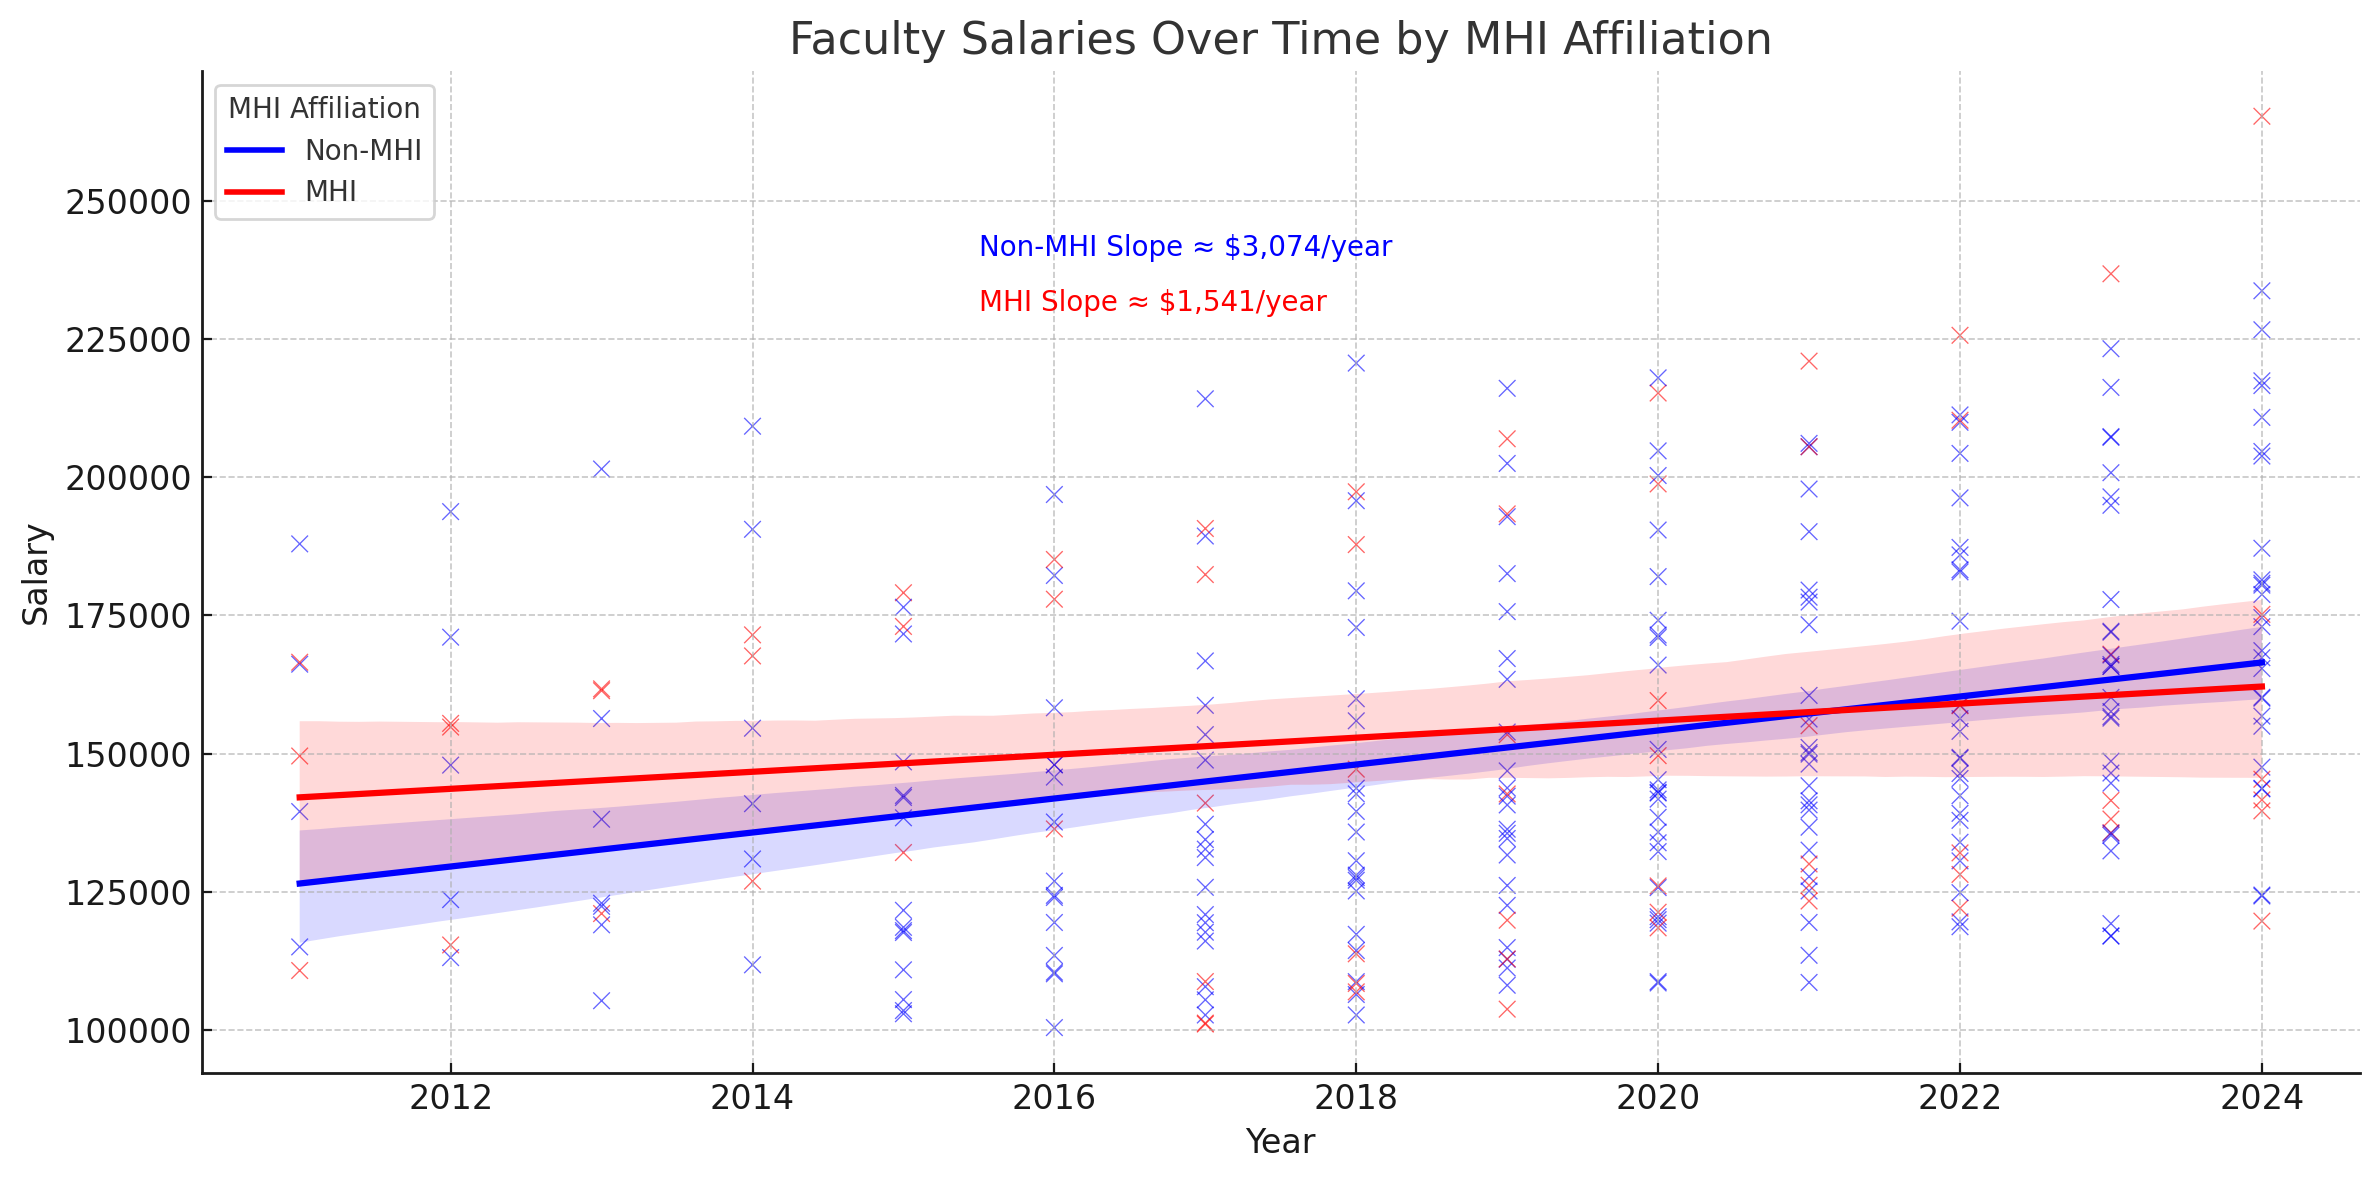
\includegraphics[width=.72\textwidth]{figures/scatter.png}
    \caption{Faculty salaries over time by MHI affiliation, with regression lines showing different growth rates.}
    \label{fig:scatter_plot}
\end{figure}

\newpage
\printbibliography

\end{document}

